% Created 2023-04-14 Fri 14:59
\documentclass[9pt, b5paaper]{book}
\usepackage{xeCJK}
\usepackage[T1]{fontenc}
\usepackage[scaled]{beraserif}
\usepackage[scaled]{berasans}
\usepackage[scaled]{beramono}
\usepackage{graphicx}
\usepackage{xcolor}
\usepackage{multirow}
\usepackage{multicol}
\usepackage{float}
\usepackage{textcomp}
\usepackage{geometry}
\geometry{left=1.2cm,right=1.2cm,top=1.5cm,bottom=1.2cm}
\usepackage{algorithm}
\usepackage{algorithmic}
\usepackage{latexsym}
\usepackage{natbib}
\usepackage{minted}
\newminted{common-lisp}{fontsize=\footnotesize}
\usepackage[xetex,colorlinks=true,CJKbookmarks=true,linkcolor=blue,urlcolor=blue,menucolor=blue]{hyperref} 
\author{deepwaterooo}
\date{\today}
\title{segmentTree}
\hypersetup{
  pdfkeywords={},
  pdfsubject={},
  pdfcreator={Emacs 28.2 (Org mode 8.2.7c)}}
\begin{document}

\maketitle
\tableofcontents


\chapter{Segment Tree与Binary Index Tree 线段树与树状数组}
\label{sec-1}
\begin{itemize}
\item 【要解决的问题:】快速区间查找:O( logN)线段树主要用于高效解决连续区间的动态查询问题,由于二叉结构的特性,使用线段树可以快速的查找某一个节点在若干条线段中出现的次数,时间复杂度为O(logN)。
\item 【其它操作效率】对应于树状数组,线段树进行更新(update)的操作为O(logn),进行区间查询(range query)的操作也为O(logn)。
\item 【缺点:空间占用大】而未优化的空间复杂度为2N,因此有时需要离散化让空间压缩。
\item 【与树状数组的区别:】与树状数组不同的是,线段树不止可以适用于【区间求和的查询】,也可以进行【区间最大值,区间最小值(Range Minimum/Maximum Query problem)或者区间异或值的查询】。
\item 【分类】:就目前的理解,暂分为两类,一类求和的,一类求最大最小值、或是位操作值(|\^{}\&)等等。权值线段树是属于哪里的?
\end{itemize}
\section{求和Sum的线段树}
\label{sec-1-1}
\subsection{327. Count of Range Sum - Hard \textbf{重点} 这几个题要好好再理解消化几遍}
\label{sec-1-1-1}
Given an integer array nums and two integers lower and upper, return the number of range sums that lie in [lower, upper] inclusive.

Range sum S(i, j) is defined as the sum of the elements in nums between indices i and j inclusive, where i <= j.
\begin{enumerate}
\item 解题思路与分析: 分治法,自底向上的解决问题
\label{sec-1-1-1-1}

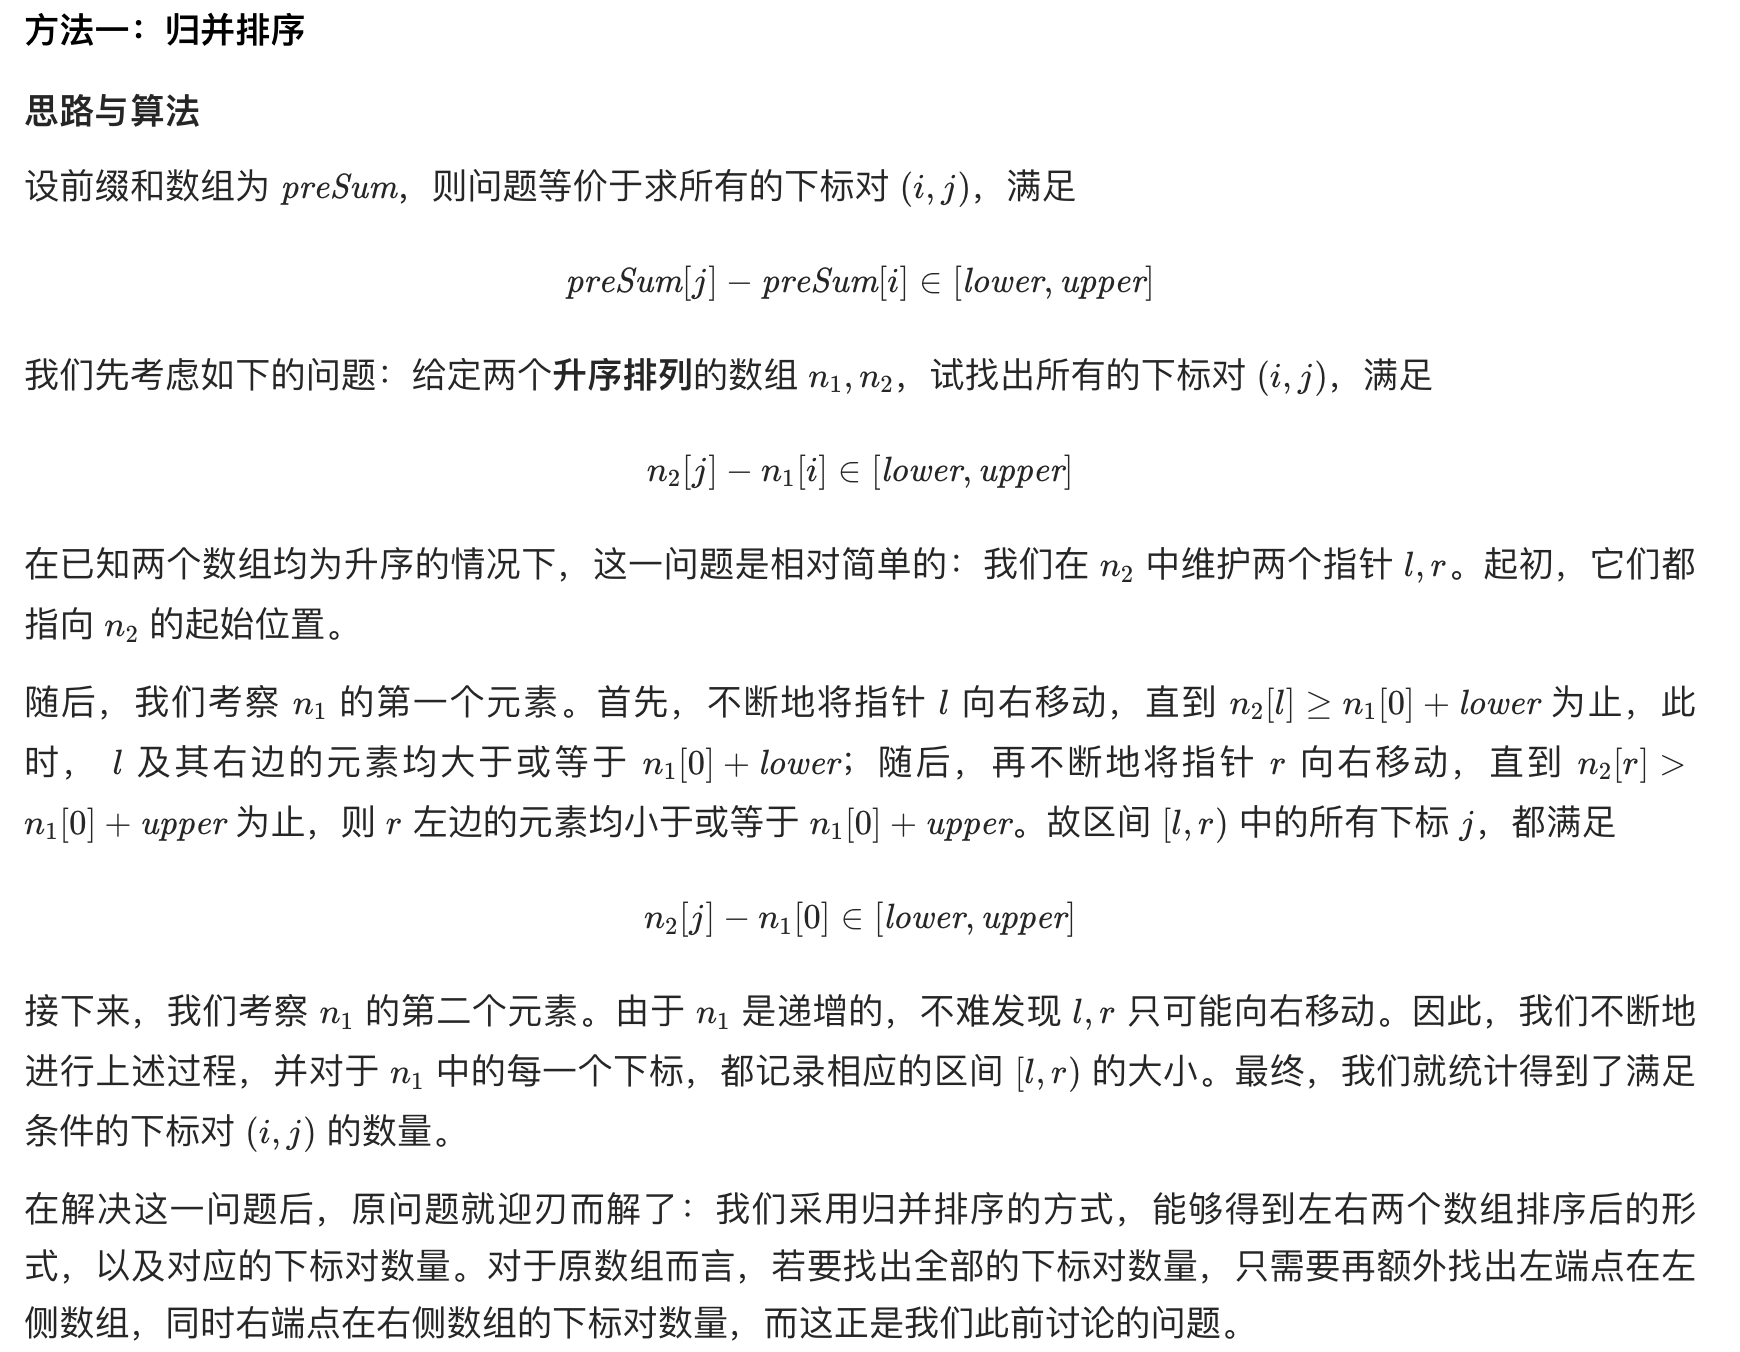
\includegraphics[width=.9\linewidth]{./pic/segmentTree_20230414_095339.png}
\begin{itemize}
\item 下面是最原始的归并排序的解法与写法
\begin{minted}[fontsize=\scriptsize,linenos=false]{java}
// 【最基本的数据结构的解法】:归并排序。整个过程是一个自底向上,不断求值与归并的过程
public int countRangeSum(int[] a, int lo, int hi) {
    int n = a.length;
    long [] s = new long [n+1]; // 用来求和 prefixSum
    for (int i = 0; i < n; i++) s[i+1] = s[i] + a[i]; // 不一定是:升序排列 
    return countRangeSumRecursive(s, lo, hi, 0, n);
}
int countRangeSumRecursive(long [] sum, int lo, int hi, int l, int r) { // l: 左下标, r: 右下标
    if (l == r) return 0;
    int m = (l + r) / 2;
    // 【首先,递归,分别解决左右半部分的问题】:分别解决了左右部分之后,左右部分分别是有序排列的片段
    int n1 = countRangeSumRecursive(sum, lo, hi, l, m);
    int n2 = countRangeSumRecursive(sum, lo, hi, m+1, r);
    int ans = n1 + n2;
    // 【再来解决归并相关】
    // 首先统计下标对的数量
    int i = l, left = m+1, right = m+1;
    while (i <= m) {
        while (left <= r && sum[left] - sum[i] < lo) left++; // 左边界右移,直到达标【 lo, 。。。
        right = left; // 可要可不要,要了可以少遍历上面的过程。。。
        while (right <= r && sum[right] - sum[i] <= hi) right++; // 右边界右移,直到不达标越界。。。 hi-1 】 hi...
        ans += right - left;
        i++;
    }
    // 随后合并两个排序数组
    long [] sorted = new long [r - l + 1];
    int x = l, y = m+1, z = 0; //x,y,z: 分别为左右两个片段的遍历下标,以及合并数组的遍历下标
    while (x <= m || y <= r) 
        if (x > m) sorted[z++] = sum[y++];
        else if (y > r) sorted[z++] = sum[x++];
        else if (sum[x] < sum[y]) sorted[z++] = sum[x++];
        else sorted[z++] = sum[y++];
    // 再把这个排序好的数组,更新同步到累积和数组里去
    for (int j = 0; j < sorted.length; j++) 
        sum[l+j] = sorted[j];
    return ans;
}
\end{minted}
\item 复杂度分析为:
\end{itemize}

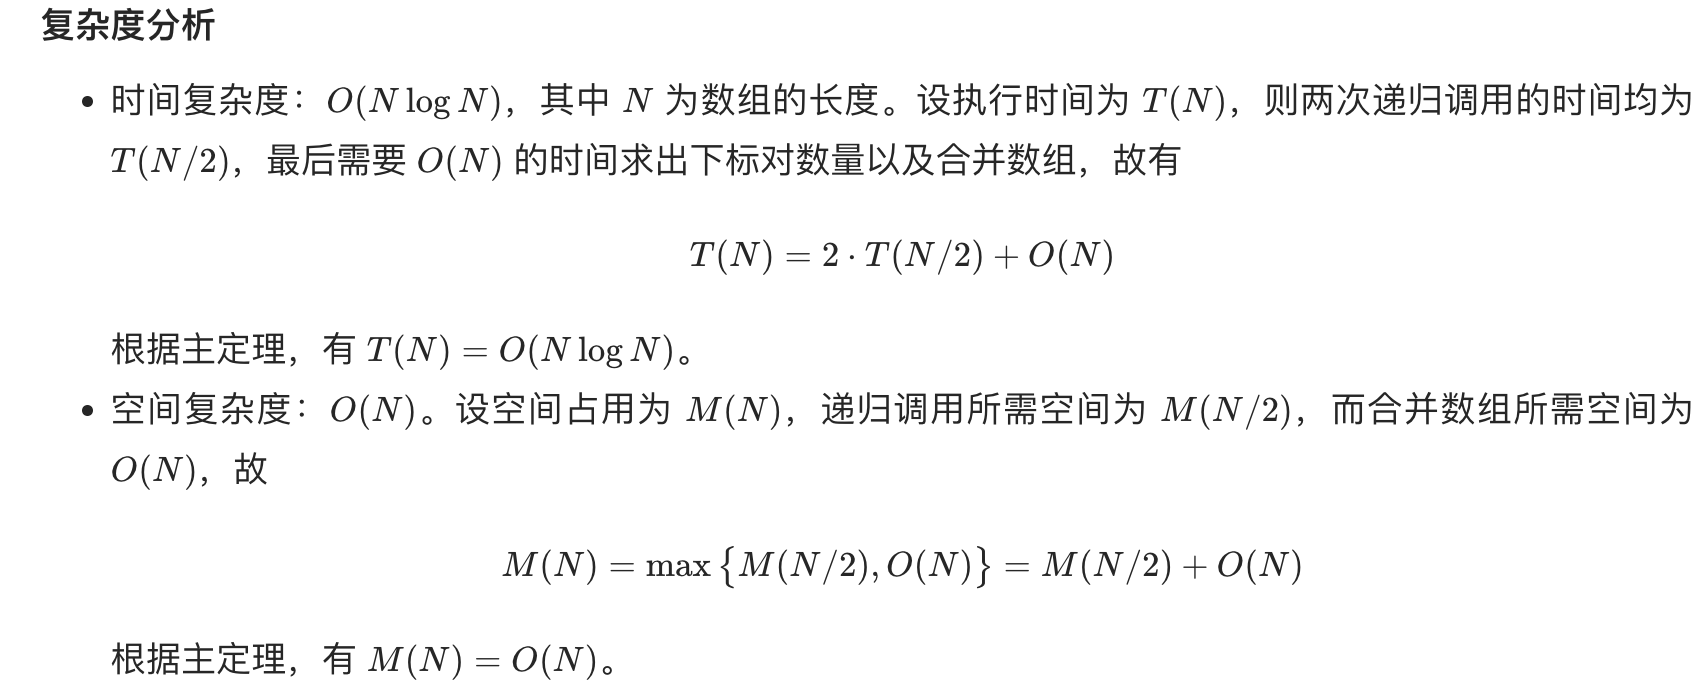
\includegraphics[width=.9\linewidth]{./pic/segmentTree_20230414_095227.png}
\begin{itemize}
\item 下面是一个代码更为简洁的写法,排序的步骤本地用语言自带的排序法
\end{itemize}
\begin{minted}[fontsize=\scriptsize,linenos=false]{java}
public int countRangeSum(int[] a, int lower, int upper) { // 这个merge sort的思维很奇特: 二分,O(NlogN)
    long [] sum = new long[a.length+1];
    for (int i = 0; i < a.length; i++)
        sum[i+1] = sum[i] + a[i];
    return mergeAnalyse(sum, 0, a.length+1, lower, upper);
}
int mergeAnalyse(long [] a, int l, int r, int lo, int hi) { // l, r: 寻找【l, r)范围内和为【lower, upper】的片段的个数
    if (r - l <= 1) return 0;
    int m = l + (r - l) / 2;
    // int mid = l + (r - l) / 2;
    // int m = mid, n = mid, ans = 0;
    int ans = mergeAnalyse(a, l, m, lo, hi) + mergeAnalyse(a, m, r, lo, hi);
    int x = m, y = m;
    for (int i = l; i < m; i++) { // 遍历[l, r)的半段长度: pivot 右移,滑动窗口,寻找合法窗口 // 通过遍历寻找当前范围中符合要求的个数,
        while (x < r && a[x] - a[i] < lo) x++; // 左端点右移,直到找到合法(sum >= lo)的解:m合法
        y = x; // 可要可不要。。。
        while (y < r && a[y] - a[i] <= hi) y++; // 右端点右移,直到右端点右移至不再合法(sum > hi), n 不合法 
        ans += y - x; // 对于[l, r)范围内的当前i来说,满足要求的总个数为 n - m
    }
    Arrays.sort(a, l, r); // 将 【l, r)片段排序,本地排序
    return ans;
}
\end{minted}
\item 解题思路与分析: 求和 sum 线段树 + 离散化数据的连续化处理
\label{sec-1-1-1-2}

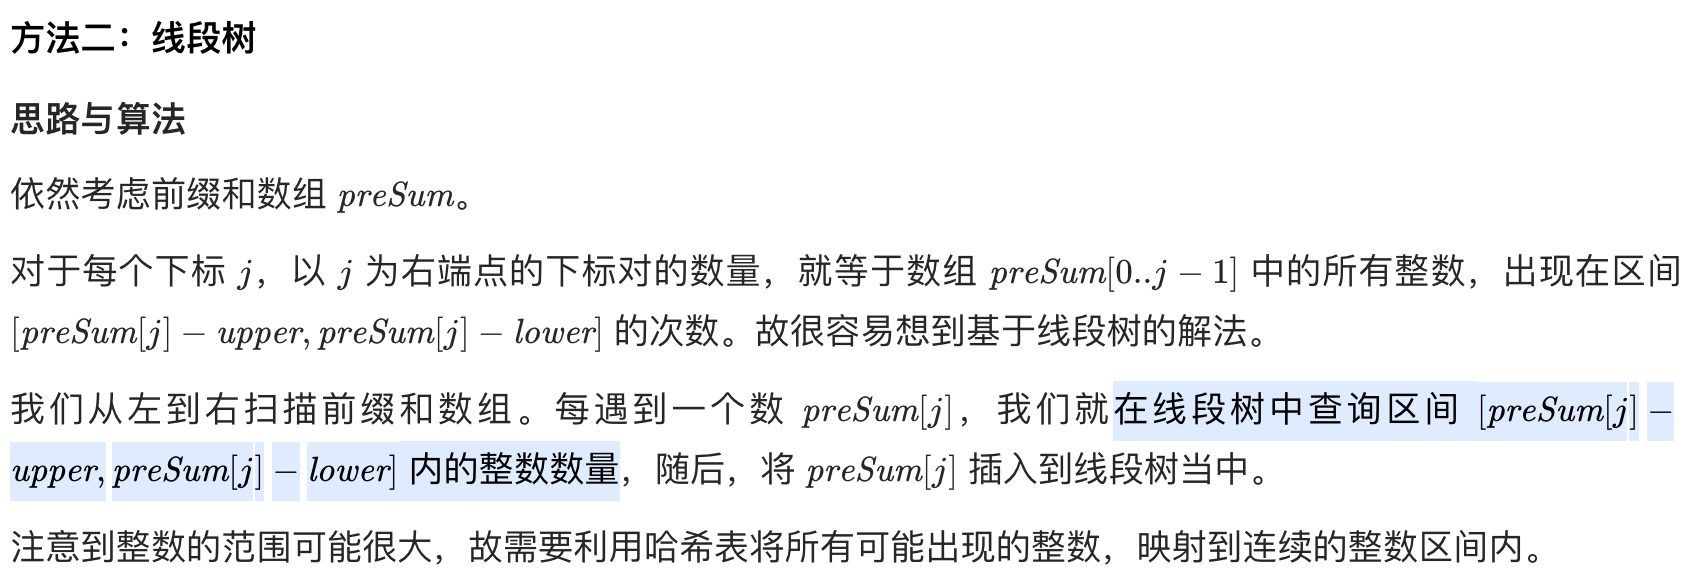
\includegraphics[width=.9\linewidth]{./pic/segmentTree_20230414_110820.png}
\begin{minted}[fontsize=\scriptsize,linenos=false]{java}
// 最基本的【求和 sum 线段树】:将前缀和数值中的取值范围,分布到Bit 的数组上来,可能需要必要的取值偏移【不是偏移,用个策略!!!】,以保证 bit 每个元素取值 >= 1
// 这里还是来参考别人更为精典的解决办法 
public int countRangeSum(int[] a, int lo, int hi) {
    int n = a.length;
    long [] s = new long [n+1];
    for (int i = 0; i < n; i++) s[i+1] = s[i] + a[i];
    // Set<Long> allNumbers = new HashSet<>(); // 考量:去重作用【BUGGLY CODING:】没有考虑到这里的排序作用。。。
    Set<Long> allNumbers = new TreeSet<>();    // 考量:去重作用【BUGGLY CODING:】没有考虑到这里的排序作用。。。【狠狠狠重要!否则不成解!!!】
    for (long v : s) {
        allNumbers.add(v);
        allNumbers.add(v - lo);
        allNumbers.add(v - hi);
    }
    // 利用哈希表进行离散化:这里离散化的本质是:将离散的取值,重新序列化为【0,n-1】下标的值序列片段!!!
    // 注意到整数的范围可能很大,故需要利用哈希表将所有可能出现的整数,映射到连续的整数区间内。
    // 【前面的离散长整形数据,如果不排列,映射到连续片段的下标计数,没有意义。。。】
    Map<Long, Integer> values = new HashMap<>();
    int idx = 0;
    for (long v : allNumbers) 
        values.put(v, idx++); // 【只有 allNumbers 排序过】:映射过来的 idx 的取值才能正确反映离散值在线段树中所处的正确位置。。。
    Node root = build(0, values.size()-1);
    int ans = 0;
    for (long v : s) {
        int l = values.get(v - hi), r = values.get(v - lo);
        ans += count(root, l, r); // 【理解困难的地方:】第一次的数个数,是什么时候,这个时候调用,会更新哪些?
        insert(root, values.get(v)); // 这里就添加了【0,n-1】下标范围内的某个下标,把离散的值连续化到一个有效片段,最小区间求和 sum 线段树
    }
    return ans;
}
// 求和 sum 线段树:三个最基本的方法:构建线段树,更新(插入一个值)线段树,查询区间内的个数
public Node build(int lo, int hi) { // 【lo,hi】:问题是,创建树的时候,没有,不曾数过、更新过每个区间的元素个数和???
    Node r = new Node(lo, hi);
    if (lo == hi) return r;
    int m = (hi + lo) / 2; 
    r.left = build(lo, m);
    r.right = build(m+1, hi);
    // r.s = r.left.s + r.right.s; // 父节点的个数 = 左右子树节点个数的和【为什么它这里没有更新?】
    return r;
}
public int count(Node r, int left, int right) { // 求和线段树:是否与BST 一样,右边节点计数大于左边与根节点呢?
    // 因为下面这一行的处理:区间外完全不用考虑,返回0
    if (left > r.r || right < r.l) return 0; // 查询区间,当前区间节点,完全不用考虑
    if (left <= r.l && r.r <= right) return r.s; // 【我是什么时候,才来更新这个计数 s 的?】
    // 所以,这里就可以直接调用,递归左右子数,求计数和
    return count(r.left, left, right) + count(r.right, left, right);
}
public void insert(Node r, int v) { // 这里可以理解为:动态更新,过程中随机增加一个元素
    r.s++; // 这个时候,才知道,计数,计算区间内元素个数,原来是如此精炒地完成的。。。
    if (r.l == r.r) return ; // 叶子节点 
    int m = (r.l + r.r) / 2;
    if (v <= m) insert(r.left, v);
    else insert(r.right, v);
}
class Node {
    int l, r, s; // 区间值的范围【l, r】
    Node left, right; 
    public Node(int left, int right) {
        l = left;
        r = right;
        s = 0;
        this.left = null;
        this.right = null;
    }
}
\end{minted}
\begin{itemize}
\item 线段树:方法的复杂度分析
\end{itemize}


\includegraphics[width=.9\linewidth]{./pic/segmentTree_20230414_110931.png}
\item 解题思路与分析: 动态增加节点的线段树
\label{sec-1-1-1-3}


\includegraphics[width=.9\linewidth]{./pic/segmentTree_20230414_113119.png}
\begin{minted}[fontsize=\scriptsize,linenos=false]{java}
class Node {
    long l, r; // 区间值的范围【l, r】
    int s;
    Node left, right; 
    public Node(long left, long right) {
        l = left;
        r = right;
        s = 0;
        this.left = null;
        this.right = null;
    }
}
public int countRangeSum(int[] a, int lo, int hi) {
    int n = a.length;
    long [] s = new long [n+1];
    for (int i = 0; i < n; i++) s[i+1] = s[i] + a[i];
    // 可以不实用哈希表进行映射,而是只在线段树的插入操作过程中动态地增加树中的节点。
    // 而当我们进行查询操作时,如果到达一个空节点,那么说明对应的区间中暂时还没有值,就可以直接返回 0
    long lowrBound = Long.MAX_VALUE, highBound = Long.MIN_VALUE;
    for (long v : s) {
        lowrBound = Math.min(Math.min(lowrBound, v), Math.min(v - lo, v - hi));
        highBound = Math.max(Math.max(highBound, v), Math.max(v - lo, v - hi));
    }
    Node root = new Node(lowrBound, highBound);
    int ans = 0;
    for (long v : s) {
        ans += count(root, v - hi, v - lo); // 【理解困难的地方:】第一次的数个数,是什么时候,这个时候调用,会更新哪些?
        insert(root, v); // 这里就添加了【0,n-1】下标范围内的某个下标,把离散的值连续化到一个有效片段,最小区间求和 sum 线段树
    }
    return ans;
}
// 求和 sum 线段树:这里精简成了,两个方法。。。因为不曾分步构建过树,所以必要的时候,必须先判断是否为空,添加节点 
public long count(Node r, long left, long right) { // 求和线段树:是否与BST 一样,右边节点计数大于左边与根节点呢?
    if (r == null) return 0;
    // 因为下面这一行的处理:区间外完全不用考虑,返回0
    if (left > r.r || right < r.l) return 0; // 查询区间,当前区间节点,完全不用考虑
    if (left <= r.l && r.r <= right) return r.s; // 【我是什么时候,才来更新这个计数 s 的?】
    // 所以,这里就可以直接调用,递归左右子数,求计数和
    return count(r.left, left, right) + count(r.right, left, right);
}
public void insert(Node r, long v) { // 这里可以理解为:动态更新,过程中随机增加一个元素
    r.s++; // 这个时候,才知道,计数,计算区间内元素个数,原来是如此精炒地完成的。。。
    if (r.l == r.r) return ; // 叶子节点 
    // int m = (r.l + r.r) / 2;
    long m = (r.l + r.r) >> 1;
    if (v <= m) {
        if (r.left == null)
            r.left = new Node(r.l, m);
        insert(r.left, v);
    } else {
        if (r.right == null)
            r.right = new Node(m+1, r.r);
        insert(r.right, v);
    }
}
\end{minted}
\begin{itemize}
\item 复杂度分析:
\end{itemize}

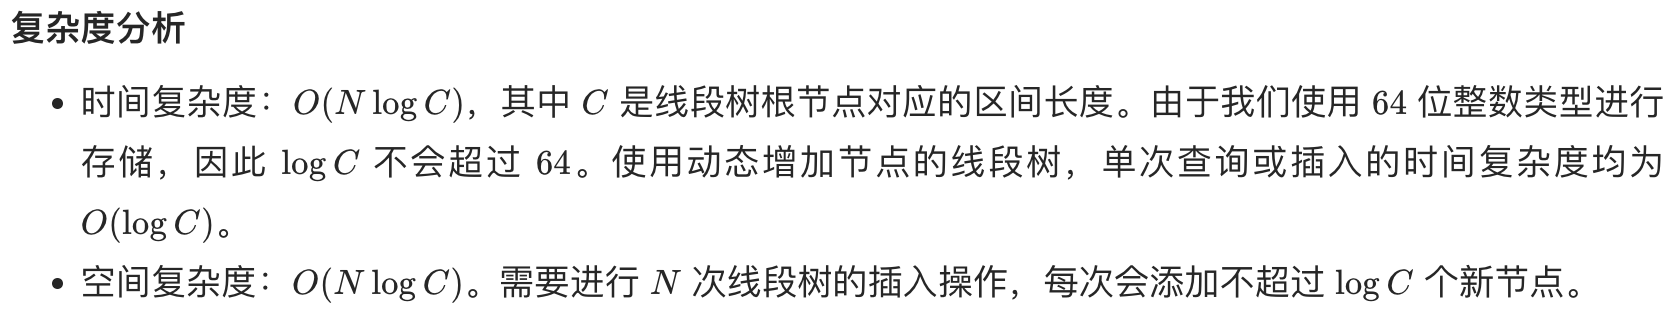
\includegraphics[width=.9\linewidth]{./pic/segmentTree_20230414_113141.png}
\item 解题思路与分析: 树状数组
\label{sec-1-1-1-4}

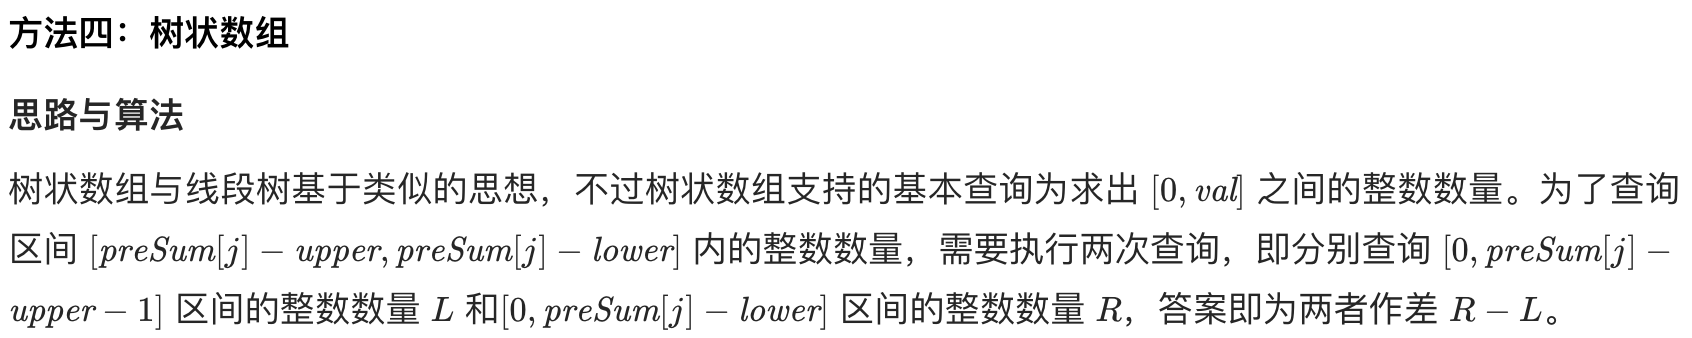
\includegraphics[width=.9\linewidth]{./pic/segmentTree_20230414_114943.png}
\begin{minted}[fontsize=\scriptsize,linenos=false]{java}
// 【方法四:】树状数组。好像我前面没能区分,线段树,与树状数组的区别?
public int countRangeSum(int[] a, int lo, int hi) {
    int n = a.length;
    long [] s = new long [n+1];
    for (int i = 0; i < n; i++) s[i+1] = s[i] + a[i];
    Set<Long> allNumbers = new TreeSet<>();
    for (long v : s) {
        allNumbers.add(v);
        allNumbers.add(v - lo);
        allNumbers.add(v - hi);
    }            
    // 利用哈希表进行离散化
    Map<Long, Integer> values = new HashMap<Long, Integer>();
    int idx = 0;
    for (long v : allNumbers)
        values.put(v, idx++);
    int ans = 0;
    BIT bit = new BIT(values.size());
    for (int i = 0; i < s.length; i++) {
        int left = values.get(s[i] - hi), right = values.get(s[i] - lo);
        ans += bit.query(right + 1) - bit.query(left);
        bit.update(values.get(s[i]) + 1, 1);
    }
    return ans;
}
class BIT {
    int [] tree; 
    int n;
    public BIT(int n) {
         this.n = n;
         this.tree = new int[n+1];
     }
    public static int lowbit(int x) {
        return x & (-x); 
    }
    public void update(int idx, int d) {
        while (idx <= n) {
            tree[idx] += d;
            idx += lowbit(idx);
        }
    }
    public int query(int x) {
        int ans = 0;
        while (x != 0) {
            ans += tree[x];
            x -= lowbit(x);
        }
        return ans;
    }
}
\end{minted}


\includegraphics[width=.9\linewidth]{./pic/segmentTree_20230414_115003.png}
\item 解题思路与分析: 平衡二叉搜索树
\label{sec-1-1-1-5}

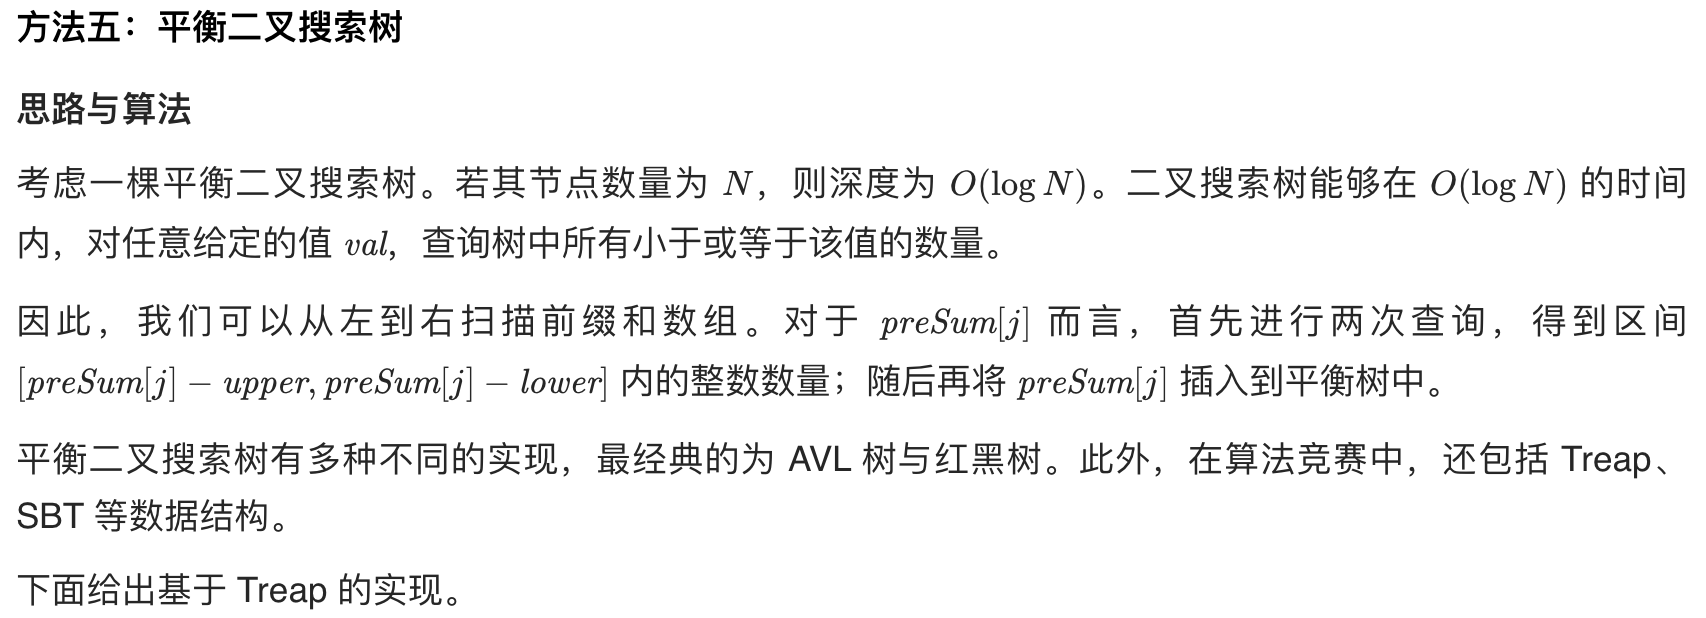
\includegraphics[width=.9\linewidth]{./pic/segmentTree_20230414_142718.png}

\begin{minted}[fontsize=\scriptsize,linenos=false]{java}
// 【方法五:平衡二叉搜索树】
public int countRangeSum(int[] a, int lo, int hi) {
    long [] s = new long [a.length+1];
    for (int i = 0; i < a.length; i++) s[i+1] = s[i] + a[i];
    BT tr = new BT();
    int ans = 0;
    for (long v : s) {
        long numLeft = tr.lowerBound(v - hi);
        int rankLeft = (numLeft == Long.MAX_VALUE ? (int)(tr.getSize()+1) : tr.rank(numLeft)[0]);
        long numRight = tr.upperBound(v - lo);
        int rankRight = (numRight == Long.MAX_VALUE ? (int)tr.getSize() : tr.rank(numRight)[0]-1);
        ans += rankRight - rankLeft + 1;
        tr.insert(v);
    }
    return ans;
}
class BT {// Treap = Tree+Heap: 
  private class Node {
        long v, s;
        int cnt, size;
        Node l, r;
        Node(long val, long seed) {
            v = val;
            s = seed; // 为什么要这个种子?伪随机数吗?【Treap 的修正值】:修正值满足最小堆性质
            cnt = 1;
            size = 1;
            l = null; r = null;
        }
        //   this         r <== root
        //  /    \      /    \
        // l      r   this   r.r(root.r)
        //           /    \
        //          l     r.l(root.l)
        Node leftRotate() { // 左旋:当前根this 变成左子节点;先前右变成根
            int prevSize = size;
            int currSize = (l != null ? l.size : 0) + (r.l != null ? r.l.size : 0) + cnt; // 左右子树的 size +当前根节点的 cnt
            Node root = r; // 这里先把 root 当作 r 的另一个索引指针
            r = root.l;
            root.l = this;
            root.size = prevSize; // 【没看明白:】是怎么变过来的?
            size = currSize;
            return root;
        }
        //       this         l <== root
        //      /    \      /    \
        //     l      r   l.l    this
        //   /    \             /    \
        // l.l    l.r         l.r     r
        Node rightRotate() {
            int prevSize = size;
            int currSize = (r != null ? r.size : 0) + (l.r != null ? l.r.size : 0) + cnt;
            Node root = l;
            l = root.r;
            root.r = this;
            root.size = prevSize; // 【没看明白:】是怎么变过来的?
            size = currSize;
            return root;
        }
    }
    private Node root;
    private int size;
    private Random rand;
    public BT() {
        this.root = null;
        this.size = 0;
        this.rand = new Random();
    }
    public long getSize() {
        return size;
    }
    public void insert(long v) {
        ++size;
        root = insert(root, v);
    }
    public long lowerBound(long v) { // 这是找,最小的一个不小于 v 【 >= v】的值吗?
        Node r = root;
        long ans = Long.MAX_VALUE;
        while (r != null) {
            if (v == r.v) return v;
            if (v < r.v) {
                ans = r.v;
                r = r.l;
            } else r = r.r;
        }
        return ans;
    }
    public long upperBound(long v) { // 找一个最大的【 <= v】的值
        Node r = root;
        long ans = Long.MAX_VALUE;
        while (r != null) {
            if (v < r.v) {
                ans = r.v;
                r = r.l;
            } else r = r.r;
        }
        return ans;
    }
    public int [] rank(long v) {
        Node r = root;
        int ans = 0;
        while (r != null) {
            if (v < r.v) r = r.l;
            else { // v >= r.v
                ans += (r.l != null ? r.l.size : 0) + r.cnt;
                if (v == r.v)
                    return new int [] {ans - r.cnt + 1, ans};
                r = r.r;
            }
        }
        return new int [] {Integer.MIN_VALUE, Integer.MAX_VALUE};
    }
    private Node insert(Node r, long v) {
        if (r == null) return new Node(v, rand.nextInt());
        ++r.size;
        if (v < r.v) { // 左子树
            r.l = insert(r.l, v);
            if (r.l.s > r.s) // 这里有步检查是否平衡的步骤?
                r = r.rightRotate();
        } else if (v > r.v) { // 右子树
            r.r = insert(r.r, v);
            if (r.r.s > r.s)
                r = r.leftRotate();
        } else ++r.cnt; // 当前根节点
        return r;
    }
}
\end{minted}
\begin{itemize}
\item 复杂度分析
\begin{itemize}
\item 时间复杂度:O(NlogN)。
\item 空间复杂度:O(N)。
\end{itemize}
\item 这里简单介绍一下Treap 这个数据结构,因为最易编程,被广泛使用,应该掌握。
\end{itemize}

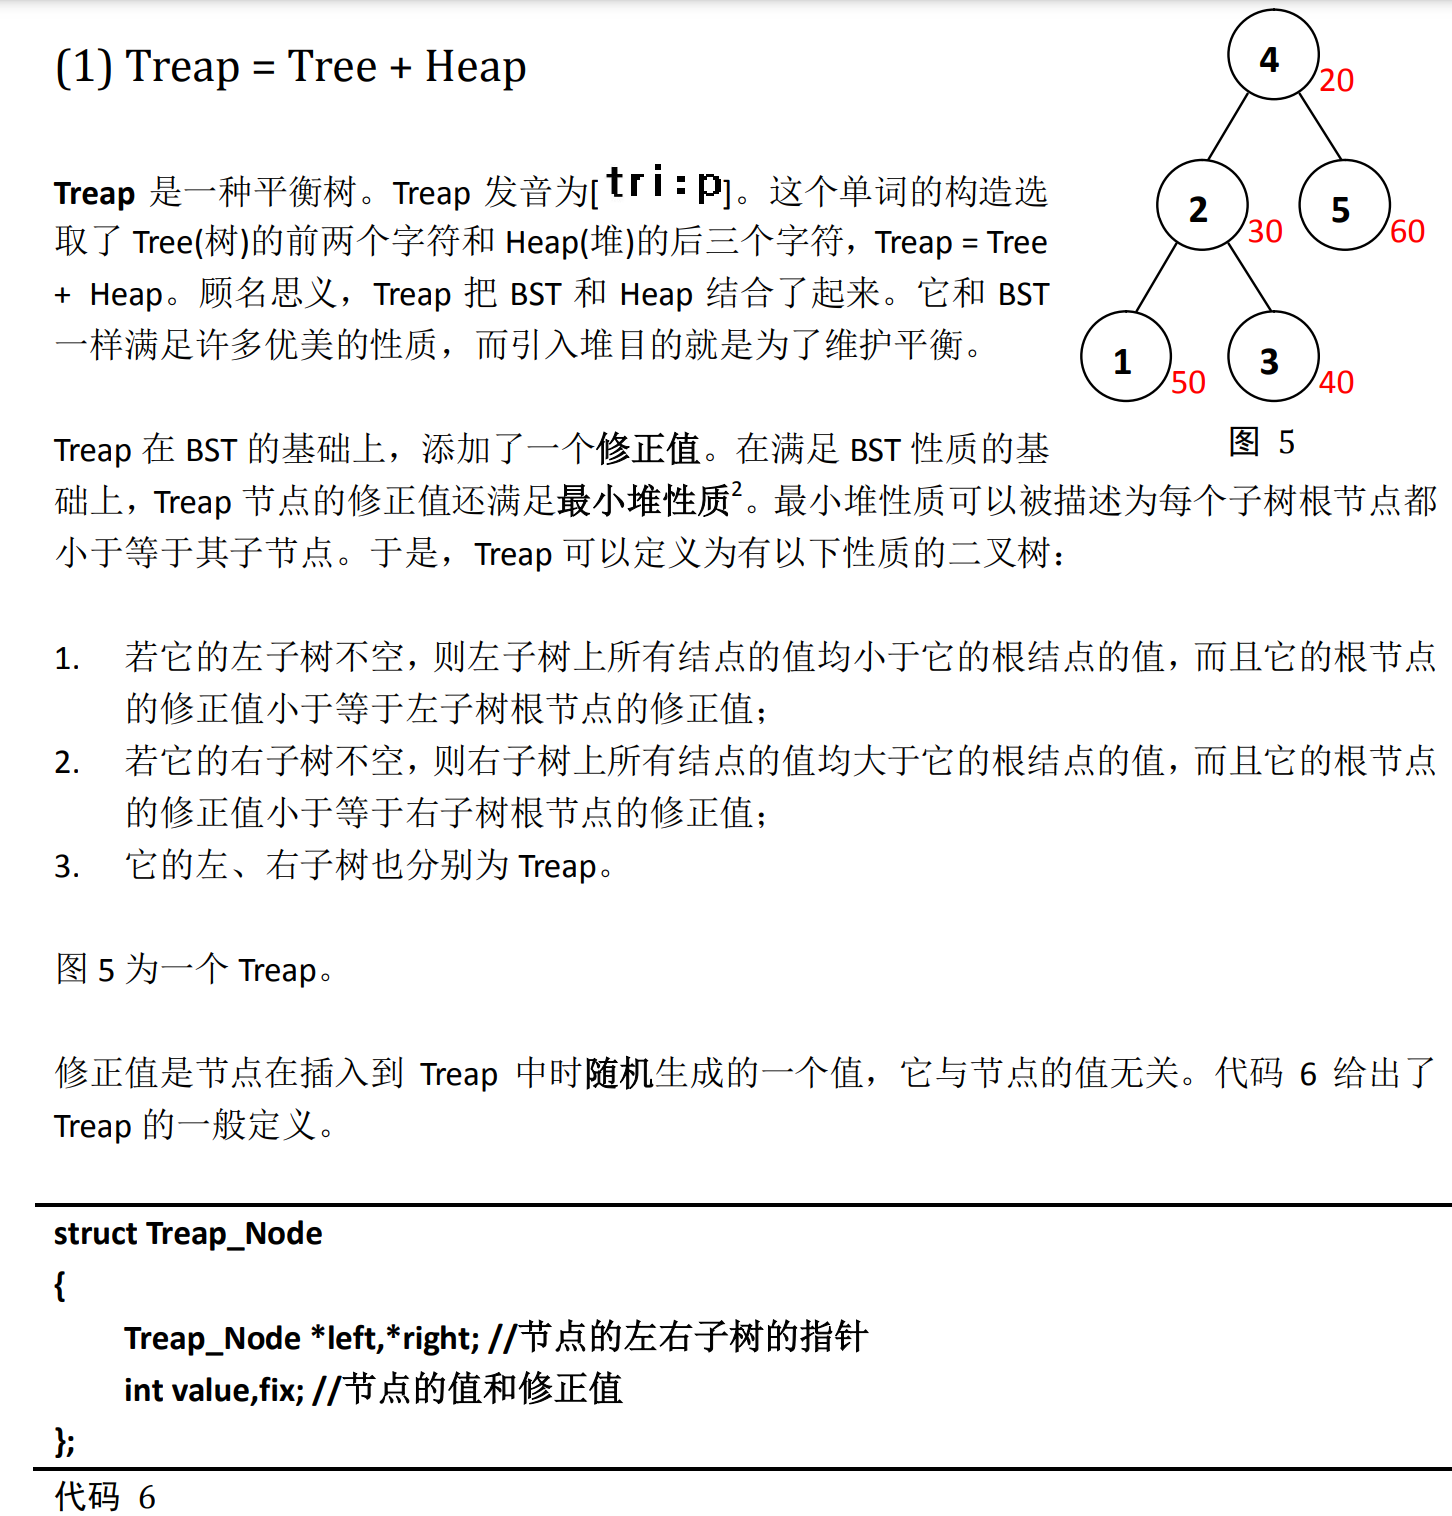
\includegraphics[width=.9\linewidth]{./pic/segmentTree_20230414_145439.png}
\begin{itemize}
\item 维护平衡的原因:修正值 
\begin{itemize}
\item 为什么平衡:我们发现,BST 会遇到不平衡的原因是因为有序的数据会使查找的路径退化成链,而随机的数据使 BST 退化的概率是非常小的。在 Treap 中,修正值的引入恰恰是使树的结构不仅仅取决于节点的值,还取决于修正值的值。然而修正值的值是随机生成的,出现有序的随机序列是小概率事件,所以 Treap 的结构是趋向于随机平衡的。
\end{itemize}
\end{itemize}
\end{enumerate}

\subsection{1157. Online Majority Element In Subarray - Hard}
\label{sec-1-1-2}
Design a data structure that efficiently finds the majority element of a given subarray.

The majority element of a subarray is an element that occurs threshold times or more in the subarray.

Implementing the MajorityChecker class:

MajorityChecker(int[] arr) Initializes the instance of the class with the given array arr.
int query(int left, int right, int threshold) returns the element in the subarray arr[left\ldots{}right] that occurs at least threshold times, or -1 if no such element exists.

\begin{itemize}
\item \url{https://www.cnblogs.com/slowbirdoflsh/p/11381565.html} 思路比较清晰
\end{itemize}

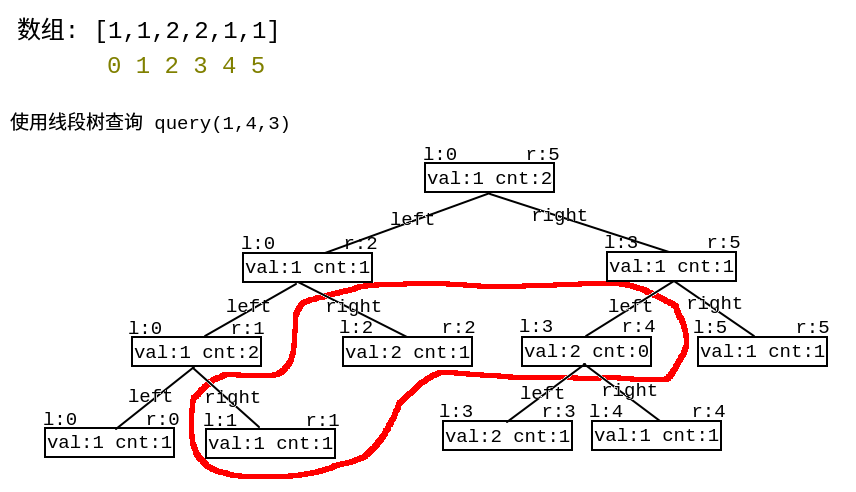
\includegraphics[width=.9\linewidth]{./pic/1157.png}

\begin{minted}[fontsize=\scriptsize,linenos=false]{java}
Map<Integer, List<Integer>> idx; // idx 存储数组出现元素种类 以及该元素下标索引
Node root; // 线段树的根节点
int key = 0, cnt = 0; // key 所查找的区域众数; count 所查找的区域众数出现次数, 
public MajorityChecker(int[] a) {
    idx = new HashMap<>(); // idx 存储数组出现元素种类 以及该元素下标索引
    for (int i = 0; i < a.length; i++)
        idx.computeIfAbsent(a[i], z -> new ArrayList<>()).add(i);
    root = buildTree(a, 0, a.length-1);
}
public int query(int left, int right, int threshold) {
    key = 0; cnt = 0; // 初始化 所查询众数key 及辅助判断的计数cnt
    searchTree(root, left, right); // 查询线段树
    // 如果查询区域没有众数 即key没被更改; 或者,
    // 所查询出来的众数 在原数组中根本没有超出阈值的能力
    if (key == 0 || idx.get(key).size() < threshold) return -1;
    // 上确界 排序数组中 第一个大于right的下标
    int r = upper_bound(idx.get(key), right);
    // 下确界 排序数组中 第一个大于等于left的下标
    int l = lower_bound(idx.get(key), left);
    cnt = r - l;
    return cnt >= threshold ? key : -1;
}
int upper_bound(List<Integer> list, int v) { // 排序数组中 第一个大于tar的下标
    int l = 0, r = list.size();
    while (l < r) {
        int mid = l + (r - l) / 2;
        if (list.get(mid) <= v) l = mid + 1;
        else r = mid;
    }
    return l;
}
int lower_bound(List<Integer> list, int v) { // 排序数组中 第一个大于等于tar的下标
    int l = 0, r = list.size();
    while (l < r) {
        int mid = l + (r - l) / 2;
        if (list.get(mid) < v) l = mid+1;
        else r = mid;
    }
    return l;
}
void searchTree(Node root, int l, int r) {
    if (root == null || l > r) return ;
    if (root.l > r || root.r < l) return ;
    if (root.l >= l && root.r <= r) { // 当查询边界被节点边界覆盖,该节点就是查询区域
        if (key == root.v) cnt += root.cnt;
        else if (cnt <= root.cnt) {
            key = root.v;
            cnt = root.cnt - cnt;
        } else cnt = cnt - root.cnt;
        return ;
    }
    int mid = (root.l + root.r) / 2; // 这两个查询条件再好好想想 !!!!!!!!!!!!!!!
    if (l <= mid)   // root.l <= l <= mid 左节点也可以是查询区域
        searchTree(root.left, l, r);
    if (r >= mid+1) // mid+1 <= r <= root.r 右节点也可以是查询区域
        searchTree(root.right, l, r);
}
Node buildTree(int [] a, int l, int r) {
    if (l > r) return null;
    Node root = new Node(l, r); // 初始一个线段树的根节点
    if (l == r) { // 叶子节点  
        root.v = a[l];
        root.cnt = 1;
        return root;
    }
    int mid = (l + r) / 2;
    root.left = buildTree(a, l, mid);
    root.right = buildTree(a, mid+1, r);
    makeRoot(root); // 整合父节点
    return root;
}
void makeRoot(Node r) { // 整合父节点
    if (r == null) return ;
    if (r.left != null) { // 如果该节点有左子节点 该节点的值"先"等于左子节点
        r.v = r.left.v;
        r.cnt = r.left.cnt;
    }
    if (r.right != null) { // 如果该节点还有右子节点 融合父节点和子节点
        if (r.v == r.right.v)
            r.cnt = r.cnt + r.right.cnt;
        else {
            if (r.cnt >= r.right.cnt)
                r.cnt = r.cnt - r.right.cnt;
            else {
                r.v = r.right.v;
                r.cnt = r.right.cnt - r.cnt;
            }
        }
    }
}
class Node {
    int l, r, v, cnt;
    Node left, right;
    public Node(int l, int r) {
        this.l = l; this.r = r;
        v = 0; cnt = 0;
        left = null; right = null;
    }
}
\end{minted}
\subsection{1825. Finding MK Average - Hard}
\label{sec-1-1-3}
You are given two integers, m and k, and a stream of integers. You are tasked to implement a data structure that calculates the MKAverage for the stream.

The MKAverage can be calculated using these steps:

If the number of the elements in the stream is less than m you should consider the MKAverage to be -1. Otherwise, copy the last m elements of the stream to a separate container.
Remove the smallest k elements and the largest k elements from the container.
Calculate the average value for the rest of the elements rounded down to the nearest integer.
Implement the MKAverage class:

MKAverage(int m, int k) Initializes the MKAverage object with an empty stream and the two integers m and k.
void addElement(int num) Inserts a new element num into the stream.
int calculateMKAverage() Calculates and returns the MKAverage for the current stream rounded down to the nearest integer.
\begin{minted}[fontsize=\scriptsize,linenos=false]{java}
// 根据题意需要找到前k大的数,又需要求区间和,就自然想到线段树.写起来较不容易出错。
// 维护2个线段树数组,一个记录数的个数,一个记录区间值,
// 注意一般线段树中[s,e]指固定的区间,这里类似线段数求第k小的数,所以[s,e]指第s小的值到第e小的值的区间。
    Deque<Integer> q = new ArrayDeque<>(); // 始终维护m个数
    int [] cnt;  // 每个元素出现的次数
    long [] sum; // 累积和
    int m, k, n = 100000, N = n * 4 + 1; // 线段树所占用的空间为数组的四倍大小
    public MKAverage(int m, int k) {
        cnt = new int [N];
        sum = new long [N];
        this.m = m;
        this.k = k;
    }
    public void addElement(int num) {
        if (q.size() == m) {
            int v = q.pollFirst();
            insert(1, 0, n, v, -1); // 当删除掉一个元素的时候,需要更新线段树中的和
        }
        insert(1, 0, n, num, 1);
        q.offerLast(num);
    }
    public int calculateMKAverage() {
        if (q.size() < m) return -1;
        int bgn = k + 1, end = m - k; // idx: 1 - based
        return (int)(query(1, 0, n, bgn, end) / (m - 2 * k));
    }
    void insert(int idx, int l, int r, int v, long d) { // d: 
        cnt[idx] += d;
        sum[idx] += d * v;
        if (l == r) return ;
        int m = l + (r - l) / 2;
        if (v <= m)
            insert(idx << 1, l, m, v, d);       // 向左子树查询
        else insert(idx << 1 | 1, m+1, r, v, d);// 向右子树查询
    }
    long query(int idx, int l, int r, int bgn, int end) { // 线段中第 bgn 个到第 end 个
        if (l == r) { // 起始和结束最多出现2次此情况 ?
            int c = end - bgn + 1;
            return (long)c * l; //
        } else if (cnt[idx] == end - bgn + 1)
            return sum[idx];
        else {
            int m = l + (r - l) / 2;
            int cl = cnt[idx << 1];     // left child cnt
            // int cr = cnt[idx << 1 | 1];     // left child cnt
            if (cl >= end) // 搜索 左 子树
                return query(idx << 1, l, m, bgn, end); 
            else if (cl >= bgn) // 搜索 左 右 子树
                return query(idx << 1, l, m, bgn, cl) + query(idx << 1 | 1, m+1, r, 1, end - cl);
            else // cl < bgn, 搜索 右 子树
                return query(idx << 1 | 1, m+1, r, bgn - cl, end - cl);
        }
    }
\end{minted}
\begin{enumerate}
\item 解题思路与分析: 三个TreeMap, 自定义TreeMap
\label{sec-1-1-3-1}
\begin{minted}[fontsize=\scriptsize,linenos=false]{java}
    CusTreeMap [] ms;
    Deque<Integer> q;
    int m, k, n;
    public MKAverage(int m, int k) {
        this.m = m;
        this.k = k;
        q = new ArrayDeque<>();
        if (m - 2 * k > 0) {
            n = 3;
            ms = new CusTreeMap[n];
            ms[1] = new CusTreeMap(m - 2 * k);
        } else {
            n = 2;
            ms = new CusTreeMap[n];
        }
        ms[0] = new CusTreeMap(k);
        ms[n-1] = new CusTreeMap(k);
    }
    // 删除num,结果总是使mapList的小、中、大三个treemap依次填充。(先保证最小的treeMap填充、再保证中间的treeMap填充、最后是最大的填充)
    private void removeElement(int num) {
        boolean removed = false;
        for (int i = 0; i < n; i++) {
            if (!removed)
                removed = ms[i].remove(num);
            else { // 将后现一两个图中的最小元素向前一个图中挪动一个数值
                Integer minK = ms[i].pollFirst();
                if (minK == null) break;
                ms[i-1].add(minK);
            }
        }
    }
    public void addElement(int num) {
        if (q.size() == m) {
            int v = q.pollFirst();
            removeElement(v);
        }
        q.offerLast(num);
        Integer vtoAdd = num;
        for (int i = 0; i < n && vtoAdd != null; i++) 
            vtoAdd = ms[i].add(vtoAdd); // 记得这里返回的是: 如果图中已有k个元素,扔出来的最大键
    }
    public int calculateMKAverage() {
        if (q.size() < m || n < 3) return -1;
        return ms[1].avg();
    }
    class CusTreeMap {
        TreeMap<Integer, Integer> m;
        final int capacity;
        int size, sum;
        public CusTreeMap(int capacity) {
            m = new TreeMap<>();
            this.capacity = capacity;
        }
        public boolean remove(int key) {
            if (m.containsKey(key)) {
                m.put(key, m.get(key)-1);
                if (m.get(key) == 0) m.remove(key);
                sum -= key;
                size--;
                return true;
            }
            return false;
        }
        public Integer pollFirst() { // return key
            if (m.size() > 0) {
                int k = m.firstKey();
                // m.remove(k); // BUG: 你也不能用原始的TreeMap.remove(),因为它会移走所有的重复(如果这个元素存在重复的话)
                remove(k); // !!!
                return k;  // 这里没有自动更新 和 
                // return m.firstKey(); // BUG: 这里并没有真正移走这个元素,只是返回了第个元素的键
            }
            return null;
        }
        public Integer add(int key) { // 返回的是删除掉元素的键
            m.put(key, m.getOrDefault(key, 0) + 1); // 这里新填入的元素是否是最后一个元素,关系不大
            size++;
            sum += key;
            if (size > capacity) {
                int last = m.lastKey();
                m.put(last, m.get(last)-1);
                if (m.get(last) == 0) m.remove(last);
                sum -= last;
                size--;
                return last;
            }
            return null;
        }
        public int avg() {
            return sum / size;
        }
    }
\end{minted}
\item 解题思路与分析: 树状数组
\label{sec-1-1-3-2}
\begin{itemize}
\item 数状数组的解法: 另外第一次看到别人 二分+树状数组也能求前k大的值。
\end{itemize}
\begin{minted}[fontsize=\scriptsize,linenos=false]{java}
// We can have a queue to maintain m elements
// Use two Fenwick tree, 1 for count and 1 for prefix sum
// Do 2 times binary search for the first k elements and the last k elements by using the count from our first fenwick tree
// We can get the sum by subtrating the sum of first k elements and sum of last k element by using our second fenwick tree
Queue<Integer> q = new LinkedList<>();
FenWick fone, ftwo;
int [] cnt = new int [100010];
long sum = 0;
int m,k;
public MKAverage(int m, int k) {
    this.m = m;
    this.k = k;
    long A [] = new long [100010];
    long B [] = new long [100010];
    fone = new FenWick(A);
    ftwo = new FenWick(B);
}
public void addElement(int num) {
    q.add(num);
    sum += num;
    fone.update(num, 1);
    ftwo.update(num, num);
    cnt[num]++;
}
public int calculateMKAverage() {
    if (q.size() < m) return -1;
    while (q.size() > m) {
        int cur = q.poll();
        cnt[cur]--;
        sum -= cur;
        fone.update(cur, -1);
        ftwo.update(cur, -cur);
    }
    // binary search for the first k (there may be duplicated)
    int l = 0, r = cnt.length-1;
    int i = -1, j = -1; // pos1, pos2 
    while (l <= r) { // 二分查找总计数
        int m = (r + l) / 2;
        long count = fone.sumRange(0, m);
        if (count >= k) {
            i = m;
            r = m -1;
        } else l = m+1;
    }
    // binary search for the last k (there may be duplicated)
    l = 0;
    r = cnt.length-1;
    while (l <= r) {
        int m = l + (r-l)/2;
        long count = fone.sumRange(m, cnt.length-1);
        if (count >= k) {
            j = m;
            l = m + 1;
        } else r = m-1;
    }
    long sum1 = ftwo.sumRange(0,  i);
    long sum2 = ftwo.sumRange(j, cnt.length-1);
    long cnt1 = fone.sumRange(0, i);
    long cnt2 = fone.sumRange(j, cnt.length-1);
    if (cnt1 > k)
        sum1 -= i*(cnt1-k);
    if (cnt2 > k)
        sum2 -= j*(cnt2-k);
    long remain = sum - sum1 - sum2; // 总和, 减去两边最小最大各K个数的和
    return (int)(remain / (m-2*k));
}
class FenWick {
    long tree []; //1-index based
    long A [];
    long arr[];
    public FenWick(long [] A) {
        this.A = A;
        arr = new long [A.length];
        tree = new long [A.length + 1];
    }
    public void update(int i, int v) {
        arr[i] += v;
        i++;
        while (i < tree.length) {
            tree[i] += v;
            i += (i & -i); // 这是的原理细节再回去复习一下
        }
    }
    public long sumRange(int i, int j) {
        return pre(j+1)-pre(i);
    }
    public long pre(int i) {
        long sum = 0;
        while (i > 0) {
            sum += tree[i];
            i -= (i & -i);
        }
        return sum;
    }
}
\end{minted}
\begin{itemize}
\item 其它比较有兴趣以的BST二叉树的解法,改天补起来
\end{itemize}
\end{enumerate}
\subsection{315. Count of Smaller Numbers After Self - Hard}
\label{sec-1-1-4}
You are given an integer array nums and you have to return a new counts array. The counts array has the property where counts[i] is the number of smaller elements to the right of nums[i].
\begin{enumerate}
\item 解题思路与分析: 二分查找的插入排序
\label{sec-1-1-4-1}
\begin{minted}[fontsize=\scriptsize,linenos=false]{java}
public List<Integer> countSmaller(int[] a) { // O(NlogN) 插入排序
    int n = a.length;
    List<Integer> ans = new ArrayList<>();
    List<Integer> list = new ArrayList<>(); // 新建一个list,用于排序
    int [] tmp = new int [n]; // 为了提高效率,新建一个数组型的返回结果
    for (int i = n-1; i >= 0; i--) {
        int v = a[i];       // 将当前数字插入到新建list中, 使用二分查找找到插入位置
        int l = 0, r = list.size()-1; // l: left; r: right 从排好序的list中二分查找正确的插入位置
        while (l <= r) {
            int m = l + (r - l) / 2;
            if (v <= list.get(m)) r = m-1;
            else l = m + 1;
         }
        list.add(l, v); // 将当前数字插入到相应位置,保证list升序排列
        tmp[i] = l; // 当前位置前所有数字均小于当前数字,将个数加入返回结果
    }
    for (Integer v : tmp) ans.add(v);
    return ans;
}
\end{minted}
\item 解题思路与分析: 数状数组
\label{sec-1-1-4-2}
\begin{itemize}
\item 官方题解: \url{https://leetcode-cn.com/problems/count-of-smaller-numbers-after-self/solution/ji-suan-you-ce-xiao-yu-dang-qian-yuan-su-de-ge-s-7/}
\begin{minted}[fontsize=\scriptsize,linenos=false]{java}
private int[] c;
private int[] a; // 离散化、去重复 后的数组
public List<Integer> countSmaller(int[] nums) {
    List<Integer> ans = new ArrayList<Integer>(); 
    discretization(nums);
    init(nums.length + 5);
    for (int i = nums.length - 1; i >= 0; --i) {
        int id = getId(nums[i]);
        ans.add(query(id - 1));
        update(id);
    }
    Collections.reverse(ans);
    return ans;
}
private void init(int length) {
    c = new int[length];
    Arrays.fill(c, 0);
}
private int lowBit(int x) {
    return x & (-x);
}
private void update(int pos) {
    while (pos < c.length) {
        c[pos] += 1;
        pos += lowBit(pos);
    }
}
private int query(int pos) {
    int ret = 0;
    while (pos > 0) {
        ret += c[pos];
        pos -= lowBit(pos);
    }
    return ret;
}
private void discretization(int[] nums) { // 离散化、去重复 ?
    Set<Integer> set = new HashSet<Integer>(Arrays.stream(nums).boxed().collect(Collectors.toList()));
    int size = set.size();
    a = new int[size];
    int index = 0;
    for (int num : set) a[index++] = num;
    Arrays.sort(a);
}
private int getId(int x) {
    return Arrays.binarySearch(a, x) + 1; // 
}
\end{minted}
\end{itemize}
\item 解题思路与分析: 归并排序 todo 补上
\label{sec-1-1-4-3}
\end{enumerate}

\subsection{699. Falling Squares - Hard}
\label{sec-1-1-5}
There are several squares being dropped onto the X-axis of a 2D plane.

You are given a 2D integer array positions where positions[i] = [lefti, sideLengthi] represents the ith square with a side length of sideLengthi that is dropped with its left edge aligned with X-coordinate lefti.

Each square is dropped one at a time from a height above any landed squares. It then falls downward (negative Y direction) until it either lands on the top side of another square or on the X-axis. A square brushing the left/right side of another square does not count as landing on it. Once it lands, it freezes in place and cannot be moved.

After each square is dropped, you must record the height of the current tallest stack of squares.

Return an integer array ans where ans[i] represents the height described above after dropping the ith square.
\begin{enumerate}
\item 解题思路与分析: O(N\^{}2) 本能土办法
\label{sec-1-1-5-1}
方块的大小不是固定的,有可能很大,但是不管方块再大,只要有一点点部分搭在其他方块上面,整个方块都会在上面,并不会掉下来,让我们求每落下一个方块后的最大高度。我们知道返回的是每落下一个方块后当前场景中的最大高度,那么返回的数组的长度就应该和落下方块的个数相同。所以我们可以建立一个heights数组,其中heights[i]表示第i块方块落下后所在的高度,那么第i块方块落下后场景的最大高度就是[0, i]区间内的最大值。那么我们在求出heights数组后,只要不停返回[0, i]区间内的最大值即可。继续来看,这道题的难点就是方块重叠的情况,我们先来想,如果各个方块不重叠,那么heights[i]的高度就是每个方块自身的高度。一旦重叠了,就得在已有的基础上再加上自身的高度。那么我们可以采用brute force的思想,对于每个一个下落的方块,我们都去看和后面将要落下的方块有没有重叠,有的话,和后面将要落下的方块的位置相比较,取二者中较大值为后面要落下的方块位置高度heights[j]。判读两个方块是否重叠的方法是如果方块2的左边界小于方块1的右边界,并且方块2点右边界大于方块1点左边界。就拿题目中的例子1来举例吧,第一个下落的方块的范围是[1, 3],长度为2,则heights\footnote{DEFINITION NOT FOUND.}=2,然后我们看其和第二个方块[2, 5]是否重叠,发现是重叠的,则heights\footnote{DEFINITION NOT FOUND.}更新为2,再看第三个方块[6, 7],不重叠,不更新。然后第二个方块落下,此时累加高度,则heights\footnotemark[2]{}=5,再看第三个方块,不重叠,不更新。然后第三个方块落下, heights\footnote{DEFINITION NOT FOUND.}=1。此时我们heights数组更新好了,然后我们开始从头遍历,维护一个当前最大值curMax,每次将[0, i]中最大值加入结果res即可,
\begin{minted}[fontsize=\scriptsize,linenos=false]{java}
public List<Integer> fallingSquares(int[][] a) {
    List<Integer> ans = new ArrayList<>();
    int n = a.length, max = 0;
    int [] hi = new int [n]; // 表示第 i 块方块落下后所在的高度
    for (int i = 0; i < n; i++) {
        int h = a[i][1], l = a[i][0], r = a[i][0] + h;
        hi[i] += h;
        for (int j = i+1; j < n; j++) {
            int ll = a[j][0], rr = ll + a[j][1];
            // [[6,1],[9,2],[2,4]] 因为不能保证是从左往下延x轴顺序掉落,所以加上l < rr 也狠重要 确保不管左右边有交叠
            if (ll < r && rr > l) // 保证j在i的右边,并且有重叠区域
                hi[j] = Math.max(hi[j], hi[i]);
        }
        max = Math.max(max, hi[i]);
        ans.add(max);
    }
    return ans;
}
\end{minted}
\item 解题思路与分析: 线段树 + 离散化
\label{sec-1-1-5-2}

想象x xx轴是地面,如果某个方块掉落的过程中遇到了之前的某个方块(擦边而过不算),则该方块会叠到上面。现在给定一个长n nn数组A AA,A [ i ] A[i]A[i]存了第i ii个掉落的方块的信息,其中A [ i ] [ 0 ] A[i]\footnotemark[1]{}A[i]\footnotemark[1]{}表示它的左下角的x xx坐标,A [ i ] [ 1 ] A[i]\footnotemark[2]{}A[i]\footnotemark[2]{}表示它的边长。要求返回一个长n nn数组B BB,使得B [ i ] B[i]B[i]表示在A [ i ] A[i]A[i]掉落之后,当前所有方块的最高点的y yy坐标。

思路是线段树 + 离散化。可以将x xx坐标离散化,这样可以节省存储空间(离散化的过程其实就是将一个数组d dd排序后去重,然后将每个数映射到它的下标。这样在线段树建树的时候,就只需维护[ 0 , l d − 1 ] [0,l\_d-1][0,l\_d−1]这个区间的信息就行了,这会极大减少线段树的空间消耗,也从而会减少要做的操作的时间消耗)。具体来说,给定一个将要下落的方块,比如该方块的左端点的x xx坐标和右端点的x xx坐标分别是a aa和b bb,边长是c cc,那么我们需要实现两个操作,第一是查询( a , b ) (a,b)(a,b)里的最大值M MM(注意这里查询的是开区间( a , b ) (a,b)(a,b)的最大值,因为下落的方块擦着另一个方块的边的话,是不会叠上去的),另一个是将[ a , b ] [a,b][a,b]里所有值都变成M + c M+cM+c。本质上是要求一个数据结构可以查询区间最大值,以及将区间修改为某一值,这可以用线段树 + 懒标记来做到。在离散化之后,为了使得区间( a , b ) (a,b)(a,b)非空(注意这里a aa和b bb都是离散化之后的值,此时( a , b ) = [ a + 1 , b − 1 ] (a,b)=[a+1,b-1](a,b)=[a+1,b−1]),我们可以在离散化的时候将方块的中点也加入一起做离散化,但是这会导致中点变成非整数,这里将原坐标乘以2 22就行了。

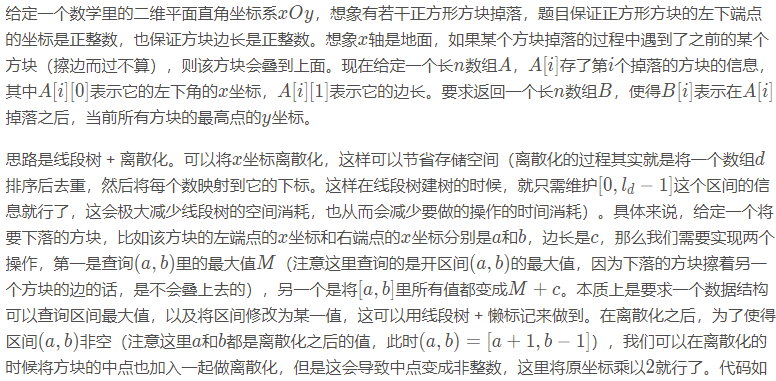
\includegraphics[width=.9\linewidth]{./pic/699.png}

\begin{minted}[fontsize=\scriptsize,linenos=false]{java}
public List<Integer> fallingSquares(int[][] a) { // 需要对数据进行离散化处理,离散化的目的是为了线段树处理起来方便;离散的是x轴的横坐标
    List<Integer> x = new ArrayList<>();
    for (int [] v : a) {
        int i = v[0], j = i + v[1];
        x.add(i * 2);
        x.add(j * 2);
        x.add(i + j);
    }
    x = getUniques(x);
    MaxSeg maxSeg = new MaxSeg(x.size());
    List<Integer> ans = new ArrayList<>();
    for (int [] v : a) {
        int i = v[0], j = i + v[1];
        i = getIdxInList(i * 2, x);
        j = getIdxInList(j * 2, x);
        int h = maxSeg.query(1, i+1, j-1);
        maxSeg.update(1, i, j, h + v[1]);
        ans.add(maxSeg.query());
    }
    return ans;
}
int getIdxInList(int v, List<Integer> list) { // 找到 x 在离散化之后的值是多少,其实就是求 xs 里 x 的下标,可以二分来找到
    int l = 0, r = list.size()-1;
    while (l < r) {
        int m = l + (r - l) / 2;
        if (list.get(m) >= v) r = m;
        else l = m + 1;
    }
    return l;
}
List<Integer> getUniques(List<Integer> l) {
    l.sort(Integer::compareTo);
    int j = 0; // 返回结果链表的下标 idx
    for (int i = 0; i < l.size(); i++) {
        if (i == 0 || l.get(j-1) != l.get(i))
            l.set(j++, l.get(i));
    }
    return l.subList(0, j);
}
class MaxSeg {   // 实现一下带懒标记的线段树 : 这棵树好强大
    class Node { // v 是 [l, r] 区间的最大值, lazy 是懒标记
        int l, r, v, lazy;
        public Node(int l, int r) {
            this.l = l;
            this.r = r;
        }
    }
    Node [] tree;
    public MaxSeg(int n) {
        tree = new Node[n << 2]; // n * 2 * 2
        buildTree(1, 0, n-1);    // 下标从 1 开始 自顶向下
    }
    void buildTree(int i, int l, int r) {
        tree[i] = new Node(l, r);
        if (l == r) return;
        int m = l + r >> 1; // (l + r) / 2
        buildTree(i << 1, l, m);
        buildTree(i << 1 | 1, m+1, r);
    }
    void pushUp(int i) { // 自底向上:自左、右叶子节点向顶更新最大值,取左右节点的最大值
        tree[i].v = Math.max(tree[i << 1].v, tree[i << 1 | 1].v);
    }
    void pushDown(int i) { // 懒标记向底、叶子方向推进一层
        int c = tree[i].lazy;
        if (c != 0) { // 打有懒标记
            tree[i].lazy = 0;
            tree[i << 1].v = tree[i << 1 | 1].v = c;
            tree[i << 1].lazy = tree[i << 1 | 1].lazy = c;
        }
    }
    void update(int i, int l, int r, int c) {   // 自顶向下传递懒标记,再自底向上更新父节点的值:取左右子节点的最大值
        if (l <= tree[i].l && tree[i].r <= r) { // 任务不需要下发,可以用懒标记懒住
            tree[i].v = tree[i].lazy = c; // 这里 tree[i].v = tree[i].lazy = c : c 是想要更新到的新值v, 用它来更新懒标记和v值
            return ;
        }
        pushDown(i);  // 任务不得不下发,则先下发给两个孩子
        int m = tree[i].l + tree[i].r >> 1;
        if (l <= m) update(i << 1, l, r, c);  // 回归调用,下传更新至左右子节点
        if (m + 1 <= r) update(i << 1 | 1, l, r, c);
        pushUp(i);  // 孩子完成了任务,再修改自己的值
    }
    int query(int i, int l, int r) {
        if (l <= tree[i].l && r >= tree[i].r) return tree[i].v;
        pushDown(i);
        int ans = 0, m = tree[i].l + tree[i].r >> 1;
        if (l <= m) ans = Math.max(ans, query(i << 1, l, r));
        if (m + 1 <= r) ans = Math.max(ans, query(i << 1 | 1, l, r));
        return ans;
    }
    int query() {
        return tree[1].v;
    }
}
\end{minted}
\item 解题思路与分析: 超简洁版的线段树,效率奇高
\label{sec-1-1-5-3}
\begin{itemize}
\item \url{http://www.noobyard.com/article/p-sxwzvpgp-nz.html}
\item 去找一下原文件中的优化步骤
\begin{minted}[fontsize=\scriptsize,linenos=false]{java}
private class Node { // 描述方块以及高度
    int l, r, h, maxR;
    Node left, right;
    public Node(int l, int r, int h, int maxR) {
        this.l = l;
        this.r = r;
        this.h = h;
        this.maxR = maxR;
        this.left = null;
        this.right = null;
    }
}
public List<Integer> fallingSquares(int[][] positions) {
    List<Integer> res = new ArrayList<>(); // 建立返回值
    Node root = null; // 根节点,默认为零
    int maxH = 0; // 目前最高的高度
    for (int[] position : positions) {
        int l = position[0]; // 左横坐标
        int r = position[0] + position[1]; // 右横坐标
        int e = position[1]; // 边长
        int curH = query(root, l, r); // 目前区间的最高的高度
        root = insert(root, l, r, curH + e);
        maxH = Math.max(maxH, curH + e);
        res.add(maxH);
    }
    return res;
}
private Node insert(Node root, int l, int r, int h) {
    if (root == null) return new Node(l, r, h, r);
    if (l <= root.l)
        root.left = insert(root.left, l, r, h);
    else
        root.right = insert(root.right, l, r, h);
    root.maxR = Math.max(r, root.maxR); // 最终目标是仅仅须要根节点更新 maxR
    return root; // 返回根节点
}
private int query(Node root, int l, int r) {
    // 新节点的左边界大于等于目前的maxR的话,直接获得0,不须要遍历了
    if (root == null || l >= root.maxR) return 0; 
    int curH = 0; // 高度
    if (!(r <= root.l || root.r <= l)) // 是否跟这个节点相交
        curH = root.h;
    // 剪枝
    curH = Math.max(curH, query(root.left, l, r));
    if (r > root.l)
        curH = Math.max(curH, query(root.right, l, r));
    return curH;
}
\end{minted}
\end{itemize}
\end{enumerate}
\subsection{1483. Kth Ancestor of a Tree Node - Hard 倍增法 binary lifting}
\label{sec-1-1-6}
You are given a tree with n nodes numbered from 0 to n - 1 in the form of a parent array parent where parent[i] is the parent of ith node. The root of the tree is node 0. Find the kth ancestor of a given node.

The kth ancestor of a tree node is the kth node in the path from that node to the root node.

Implement the TreeAncestor class:

TreeAncestor(int n, int[] parent) Initializes the object with the number of nodes in the tree and the parent array.
int getKthAncestor(int node, int k) return the kth ancestor of the given node node. If there is no such ancestor, return -1.
\begin{enumerate}
\item 解题思路与分析: 倍增 binary lifting
\label{sec-1-1-6-1}

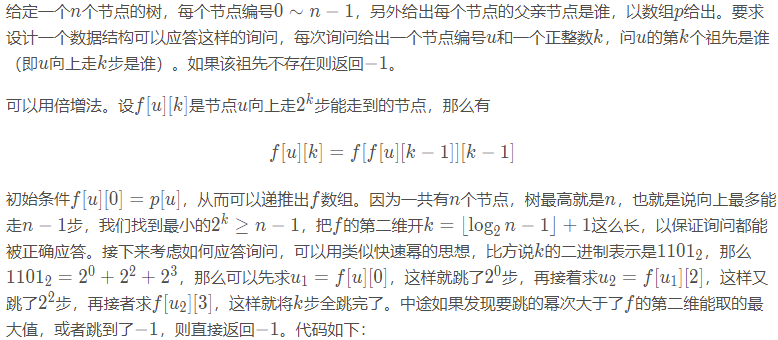
\includegraphics[width=.9\linewidth]{./pic/1483.png}

\begin{itemize}
\item 预处理时间复杂度O(nlogn),每次询问时间O(logn),空间O(nlogn)。

\begin{minted}[fontsize=\scriptsize,linenos=false]{java}
    private int [][] p;
    private int log;
    public TreeAncestor(int n, int[] parent) {
        log = (int) (Math.log(n - 1) / Math.log(2)) + 1;
        p = new int[n][log];
        for (int i = 0; i < parent.length; i++) // 初始化p数组
            p[i][0] = parent[i];
        for (int i = 1; i < log; i++) // 按公式递推p数组
            for (int j = 0; j < n; j++) 
                if (p[j][i-1] != -1) 
                    p[j][i] = p[p[j][i-1]][i-1];
                else p[j][i] = -1;
    }
    public int getKthAncestor(int node, int k) {
        int pow = 0;
        while (k > 0) {
            if (pow >= log || node == -1) return -1;
            if ((k & 1) == 1) 
                node = p[node][pow];
            k >>= 1;
            pow++;
        }
        return node;
    }
\end{minted}
\end{itemize}
\item 解题思路与分析
\label{sec-1-1-6-2}
\begin{minted}[fontsize=\scriptsize,linenos=false]{java}
    Map<Integer, List<Integer>> adj;
    int [][] par;
    public TreeAncestor(int n, int[] parent) {
        par = new int [n][30]; // 30 , 16: 不能证它是一棵很平衡的二叉树
        adj = new HashMap<>();
        for (int i = 0; i < n; i++) {
            Arrays.fill(par[i], -1);
            adj.put(i, new ArrayList<>());
        }
        for (int i = 0; i < parent.length; i++) 
            if (parent[i] != -1) {
                adj.get(parent[i]).add(i); // 自顶向下: 父 --》子节点
                par[i][0] = parent[i];     // 每个子节点的第一个父节点(2^0 = 1),即为父节点 // 自底向上: 子节点: 2^0父节点、 2^1节点、 2^2节点
            }
        dfs(0);
    }
    public int getKthAncestor(int node, int k) {
        for (int i = 0; k > 0; i++, k >>= 1) // k /= 2
            if ((k & 1) == 1) {
                node = par[node][i];
                if (node < 0) return -1;
            }
        return node;
    }
    private void dfs(int idx) { // 自顶向下:从父节点遍历子节点
        for (int i = 1; par[idx][i-1] >= 0; i++) // 穷追塑源:一直找到整棵树的根节点: 0
            par[idx][i] = par[par[idx][i-1]][i-1]; // 这里多想想
        for (int next : adj.get(idx)) 
            dfs(next);
    }
\end{minted}
\end{enumerate}
\subsection{236 二叉树的最近公共祖先}
\label{sec-1-1-7}

\subsection{1505. Minimum Possible Integer After at Most K Adjacent Swaps On Digits - Hard BIT树状数组}
\label{sec-1-1-8}
You are given a string num representing the digits of a very large integer and an integer k. You are allowed to swap any two adjacent digits of the integer at most k times.

Return the minimum integer you can obtain also as a string.
\begin{enumerate}
\item 解题思路与分析
\label{sec-1-1-8-1}
\begin{minted}[fontsize=\scriptsize,linenos=false]{java}
public String minInteger(String t, int k) {
    int n = t.length();
    t = " " + t;
    char [] s = t.toCharArray();
    ArrayDeque<Integer> [] q = new ArrayDeque [10];
    for (int i = 1; i <= n; i++) {
        int j = s[i] - '0';
        if (q[j] == null) q[j] = new ArrayDeque<>();
        q[j].offerLast(i);
    }
    BIT bit = new BIT(n);
    StringBuilder sb = new StringBuilder();
    for (int i = 1; i <= n; i++) {
        for (int j = 0; j < 10; j++) { // 从小数值往大数值遍历
            if (q[j] == null || q[j].isEmpty()) continue;
            int top = q[j].peekFirst(), pos = top + bit.sum(top); // pos是最优解的位置,最优解的位置是原来的位置加上偏移量
            if (pos - i <= k) {
                k -= pos - i;
                sb.append(j);
                q[j].pollFirst();
                bit.add(1, 1); // 更新[1, t)这段的值每个加1,即向右偏移1位.为什么要 从1开始更新:假装每次都移动到最前端,方便计算 ?
                bit.add(top, -1);
                break;
            }
        }
    }
    return sb.toString();
}
class BIT { // 开一个树状数组类,维护每个位置的字符的向右的偏移量 ? 向左偏移量
    private int n;
    private int [] a;
    public BIT(int n) {
        this.n = n;
        this.a = new int [n+1];
    }
    public void add(int idx, int v) { // 只有发生偏移,才移动某段区间的值
        while (idx <= n) {
            a[idx] += v;
            idx += lowbit(idx);
        }
    }
    public int sum(int idx) { // 得到以 i 为下标1-based的所有子、叶子节点的和, 也就是[1, idx]的和,1-based
        int ans = 0;
        while (idx > 0) {
            ans += a[idx];
            idx -= lowbit(idx);
        }
        return ans;
    }
    int lowbit(int x) {
        return x & -x;
    }
}
\end{minted}
\end{enumerate}

\section{求最大最小值、位操作值的线段树}
\label{sec-1-2}
% Emacs 28.2 (Org mode 8.2.7c)
\end{document}